\documentclass{article}
\title{Optimizing Home Design}
\author{Matthew Peyton Chenette}
\date{\today}

\usepackage{graphicx}

% TURN THIS OFF ONCE THE DOCUMENT IS FINALIZED
\usepackage{hyperref}
\hypersetup{colorlinks=true}

\begin{document}

\maketitle
\clearpage
\tableofcontents
\clearpage

\section{Introduction}
This aims to be a generic document for all houses anywhere. When and where there are preferable options for different locations, those will be noted.

This is intended to be a living document of the ideas I would like to see in a house. Many of these items were discovered or thought of after owning my first house, as well as seeing many of the houses my friends and family have lived in over the years.

Feel free to reference, reuse and redistribute this information as desired.

I am not recommending or endorsing any of the ideas below.  
I am not responsible for the consequences of applying these ideas to your house.

Should we mention that this is also intended to be a multi-generational house as to increase eco-friendliness and decrease the need for more houses and apartment buildings. also it is healthier, generally speaking, for families to be co-located with ample room in the house. so maybe talking in the ballpark of 5-7k square feet. Keeping this in mind, may be a 2 story dome (semi-sphere) on 1-2 acres

\clearpage

\section{Principles}
The principles listed below are the drivers behind each subsequent \hyperref[ideas]{idea}. Each idea is tied to one of the following principles. Doing so ensures that the house will...

% the house, during design, will...
% maximize
%   - safety
%   - natural light
% minimize
%   - footprint
%   - the possibility of bugs
%   - shocks and stresses of future events

% the house, during construction, will...
% maximize
%   - natural building materials
% minimize
%   - cutting corners

% the house, after construction, will...
% maximize
%   - natural light

\begin{enumerate} %\large \color[rgb]{0,0.5,0}
  \item maximize
  \begin{enumerate}
     \item safety (including child-proof)\label{safety}
     \item natural light \label{light}
     \item natural building materials \label{natural}
     \item utility \label{utility}
     % \item employ minimal design where possible (doorstop on hinge, etc.) using utility above instead
     \item longevity \label{longevity} % use instead of futureproof
     \item thermal mass? \label{thermalmass}
  \end{enumerate}

  \item minimize
    \begin{enumerate}
     \item maintenance \label{maintenance}
     \item recurring costs \label{cost}
     \item bugs \label{bugs}
     % \item shocks and stresses of future events \label{future-proof}
     \item cutting corners during construction \label{skimping} %call it skimping?
     \item environmental and ecosystem impact \label{environment}
  \end{enumerate}

% one for makes cleaning easier?

% maybe sections for home maintenence vs home build? or the home itself vs things in the home?

\end{enumerate}

% the tighter, more compact, more spherical the envelope/footprint, the more efficiant the house will be heating and cooling wise. Example, do not make the "workshop" an appendage that is essentially a standalone room that barely attaches to the house. It will not be efficiant to heat/cool
% no paint??? (natural)
% ivy on outdoor walls? (better for heat??)
% no drywall

%generator???
%  no generstor. We will have a ginat battery bc solar panels and the thought is that the house will be so efficient that no generator will be needed. the house can run for many days just off of the battery
% ac dampers?
% rain collection system?

% safe room,
%hidden passages
%radiant heating/cooling... no central air

% no driveway. Help with temp regulation, more visually pleaseing, less to maintain and pay for and less to go wrong. Just terraform, and use dirt/grass to flatten the area that would be a driveway

% during construction, no cutting down trees

% honestly best case scenario would be to build the house into the natural ground. Could be underground, could be into the side of a hill or mountain, could also be under a "man-made" hill, hobbit style. THis would be more natural, help with temp regulation, maintenece might be more
\clearpage
\subsection{Descriptions}
\begin{description}

\item[\ref{future-proof}] - when and where possible, use things that are not tightly integrated into the household but are modular and can be replaced as newer versions come out; also easily allowing for expansion where it is deemed likely that it may be needed in the future and where it will not require a complete refactoring of a section of the house  
\item[\ref{maintenance}] - makes cleaning easier too
\item[\ref{cost}] - ex. power/water/taxes/insurance/etc. This includes preparing for and preventing the need for all types of insurance (flood, fire, homeowners, etc.); optimized energy cost; (ex. minimize energy consumption with things like manual mower (preferring manual labor over energy spend), solar, buy media, ...)  
\item[\ref{safety}] - baby/child/family friendly and as safe as possible for all stages of life, no after-build customization needed should be able to fit a family of 5 with in-laws (i.e., +4), comfortably ; to me this also means, where- and whenever possible, no sharp edges or corners or stairs or step-downs
\item[\ref{utility}] - why have to 2 things to perform 2 tasks when you could integrate them together and just have 1 thing performing 2 tasks. ex. Tesla solar roof vs solar panels and a roof. or an integrated doorstop/door hinge instead of having them separate  
\item[\ref{synthetic}] - The building materials should be as natural as possible. all natural materials where possible, nothing that is toxic  
\item[\ref{longevity}] - This will be achieved through quality building materials and practices, not cutting corners, a acute attention to detail and to making sure we are not choosing any technology or theme/design that cannot be easily refitted or replaced 
\end{description}

\clearpage
\section{Ideas} \label{ideas}

\subsection{Construction}
\subsubsection{Framing}
\paragraph{Steel Framing}
Steel framing for the house as oppose to wood. \ref{skimping}. The idea here is that steel framing is better than wood framing in all ways except for it's thermal insulating properties, with the only trade-off being costing more than wood. This being said if I'm able to become fire resistant, bug resistant, and rot resistant at a higher price tag and with some extra focus and precision on my insulation installation, then that is the right answer.

\subsubsection{Slab}
higher slab than usual to prevent bugs? 5+in? what are the downsides?

\subsubsection{Plumbing}
\paragraph{Copper Piping}
Due to the ... the entire house should utilize copper piping, not PVC. \ref{natural} \ref{skimping} \ref{longevity}

\paragraph{No External Piping}
Keeping all piping inside the boundaries of the home's thermal envelope helps prevent burst pipes due to freezes etc and helps increase the thermal mass (\ref{thermalmass}) of the house.

Also, for external hose connections: \href{https://www.homedepot.com/p/AQUOR-1-2-in-NPT-Inlet-and-3-4-in-Faucet-Hose-Connector-4-in-House-Hydrant-V1-Modern-Outdoor-Wall-Faucet-HHP004-HD/326637204?source=shoppingads&locale=en-US&gQT=1}{home depot link}
\href{https://www.aquorwatersystems.com}{aquor water systems}

\begin{figure}
    \centering
    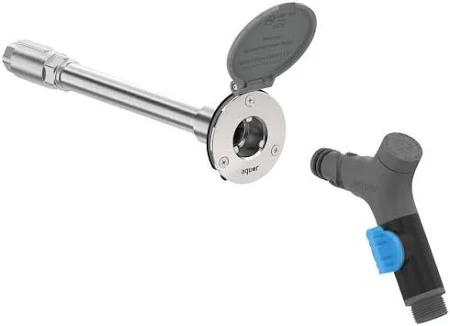
\includegraphics[width=0.5\linewidth]{image.png}
    \caption{Enter Caption}
    \label{fig:enter-label}
\end{figure}

\subsection{House}
\subsubsection{General}
thermal mass everywhere possible and to the fullest extent possible

no gutters, just concrete guides in the ground to guide the water dripping off the roof into a drain. Looks better.

\paragraph{Muted tones, colors and design decisions}
muted tones and colors, nothing bold on interior or exterior. no statements. minimal but aesthetic. natural. Future-proof! (\ref{longevity}) Bold statements fall out of taste quickly! The things listed above are safe and easy to fit into different styles

\paragraph{Misc}
4\textpm 1 bed and 3\textpm 1 bath excluding the office listed below.

\paragraph{One Story House}
A one story house is a multi-faceted win on many fronts. For one it directly addresses \ref{maintenance} and \ref{cost} as there is quite literally less house to maintain and pay for. Less taxes due to lower property valuation, less HVAC needed, etc. Also safer (no stairs) so \ref{safety}

\paragraph{Windows}
Wooden \href{https://en.wikipedia.org/wiki/Window_shutter}{Window Shutters}. Addresses \ref{safety} and \ref{utility} and kinda \ref{natural}. Also this would be in place of \href{https://en.wikipedia.org/wiki/Window_blind}{window blinds}

\paragraph{Flooring}
No carpet (or tile IMO). Only natural material rugs where desired. This allows flexibility going forward and is easier to maintain and clean. Future-proof! \ref{future-proof}
Either natural, untreated, unfinished wood (i.e., something without chemicals - \ref{synthetic}) or natural stone (i.e., slate, limestone, sandstone, etc.) and \href{https://en.wikipedia.org/wiki/Lime_mortar}{lime mortar}. For either option: aim for it to be completely flat (rather than regular tile that dips where the grout is) for easier cleaning. For wood, see \href{https://en.wikipedia.org/wiki/Wood_preservation#Charring}{Wood Preservation - Charring} and \href{https://en.wikipedia.org/wiki/Yakisugi}{Yakisugi}.
ChatGPT (JAN 2025) says, for unfinished, natural wood, make sure it is kiln-dried but otherwise untreated. ChatGPT (JAN 2025) also says: "[Natural stone flooring is] the most durable, low-maintenance natural option. Ideal for homes where longevity and minimal upkeep are priorities."

Also, apparently stone or tile is better in warmer climates as it keeps cool. better energy efficiency apparently. IDK ask ChatGPT (Jan 2025).

dedicated server room
\begin{itemize}
    \item with server rack
    \item ultra air conditioned
\end{itemize}

Last:
\begin{itemize}

\item \ref{skimping} at least one Ethernet plug in each room
\item \ref{skimping} power outlets in the floor where it's relevant (living room)
\item \ref{skimping} ceiling fan in each room
\item screened in back porch
\end{itemize}


\subsubsection{Living Room}
\paragraph{Fireplace}
No Fireplace. Less to maintain/clean/upkeep. Do not have to pay for wood or gas for it. Also it's not needed or practical in Texas. I also feel like this would give us more flexibility in the home design process as far as home layout. Kind of addresses \ref{maintenance} and \ref{cost}


\subsubsection{Kitchen}
\paragraph{Appliances}
No dishwasher - dishwashers are another source of maintenance, possible failure, hazard and potential child unsafety. Plus, most dishwashing detergents are not natural and are harmful to the gut. Plus eliminating a dishwasher eliminates the cost of dishwasher tabs every month.
\paragraph{}
No handles on cabinets - \ref{utility}? Not really it would be more like employing minimal design.\\
all electric. this includes:
    - an induction stove, no natural gas \ref{safety} \\
\href{https://youtu.be/npPhvvmTyWM?t=600}{Countertops overhang drawers by 3/4"}

40 or more inch high counter tops. This is more childproof as they wont be at risk of running into the counter tops once they can walk up to about 2-3 years. Also rounded corners on all countertops, no sharp corners.

trash can built into the cabinets or a dedicated trash can drawer. we don't just want the trashcan sitting in the walkway.

no built ins? all furniture instead? might give the space modularity so things can be moved around, the room can be rearranged or refitted. plus allows us to easily replace furniture or appiances in the future. future-proof?

no built ins? furtitur and modular choices only in case we want to rearrrange or change aeesthetic in the future?

\begin{figure}
    \centering
    \includegraphics[width=1\linewidth]{IMG_7710.png}
    \caption{Enter Caption}
    \label{fig:enter-label}
\end{figure}

\subsubsection{Office}
Office needs to be easily able to triple as either a WFH office, a "study" (like a library type setting where you don't necessarily do your computer work during the day but you can lounge/relax/read) or a bedroom (i.e. guest bedroom, another child's bedroom, or other). Needs to be flexible to be future-proof. Also no built in book shelves or anything like that anywhere. If you want bookshelves, have them be stand alone (modular). That way we can move then and easily repurpose the room if need be.

\subsubsection{Bathroom}
\paragraph{Shower} Walk in shower. Should not have step up or down to get in. Should be a lot like the one from the build show YT video. Also no door or enclosure. Walk in walk out with smooth decline into. We also need intuitive towel holder placement. Need to be easy to reach from within or just outside the shower. Could even be within the shower.

\paragraph{Bath} If even installing a bath, make it a standalone bath? not integrated into the walls/floor? thought it its easier to clean underneath, can be moved if desired, one less place for bugs to hide nest? I think it might be called a standalone bath. like \href{https://upload.wikimedia.org/wikipedia/commons/2/23/Clawfoot_bathtub.jpg}

\subsubsection{Miscellaneous}
\href{https://en.wikipedia.org/wiki/Doorstop#/media/File:Waterson-door-stop.jpg}{doorstops on hinges}. This addresses \ref{utility}

\subsection{Workshop}
- is essentially another room in the house but is MUCH bigger and has the look and feel of a 3 car garage (ex. epoxied floor, ...)
    - should be completely sealed off from outside and be a/c'd. but should likely not have its output be put into the house. So maybe a separate AC unit???. This is because if we are working with chemicals. should have a door or two that leads directly outside but is very well sealed
	- should also have the manual metal roll up workshop doors (that are like garage doors but different) that are still completely sealed off from the outside so that when they are closed, there is no a/c loss or bugs let in.
- vent hood in garage?
- drain on floor of garage
- sink in garage

\subsection{Garage}
- 2 car garage that is purely for parking in, nothing fancy
- also workshop, see that section
- regular staircase to attic (like open a door, walk up stairs), not pull down ladder

\subsection{Yard}
\subsubsection{General}
Enough land that we have neighbors but they don't live 10 feet away. we want neighbors but we don't want them to be too close
    - likely 1-2 acres of land
    - not in a flood plane + drainage of yard has been verified (flood proof)
        - \ref{cost} thus no flood insurance needed
- \ref{natural} lots of plants / green
- \ref{cost} ag or religious exemption?
\subsubsection{Extras}
\paragraph{No Pool} A pool is a safety hazard (\ref{safety})  and is costly (\ref{cost}) and time-consuming to maintain (\ref{maintenance}).

\subsubsection{Irrigation}
\paragraph{No Sprinkler System} This minimizes human impact on the environment / ecosystem (\ref{environment}) and minimizes maintenance (\ref{maintenance}) and cost (\ref{cost}).

\subsubsection{Enclosure}
% not mentioning cost for fence as there is really no recurring cost other then the maintenance %
\paragraph{No Fence} no fence means no maintenance (\ref{maintenance}), less possibility for bugs (\ref{bugs}), more visually pleasing (less clutter). there's really just no need for it. if neighbors aren't close, privacy is a non-argument, and safety is a non-argument. just use cameras. people can hop a fence

\subsubsection{Driveway}
% \paragraph{rebar in driveway/concrete} \ref{skimping}
\paragraph{No Driveway / Grass Driveway}
No concrete except for house slab? dirt driveway? More natural? maybe like \href{https://i.pinimg.com/originals/46/4f/81/464f810811fef0bcdbaa828911b20c93.jpg}{this?}
\href{https://www.truegridpaver.com/natural-driveway-ideas/}{Grass Driveway Idea}.

\subsubsection{Grass}
% Bermuda grass
Potentially buffalo grass. Or really any grass that does not require additional water other than natural rain. Any native grass. Read the \href{https://www.riveroaksgc.org/rocg-garden-book/}{Gulf Coast Gardening book} for more info.
Or maybe natural landscaping so we don't have to mow a yard?

\subsubsection{Trees}
House mostly shaded by trees? what about solar roof? large yard so house can be shaded and still have room for sun?

\subsubsection{Misc}
I like the front of the house facing west and the back/living room area facing the est for sunrise. the thought is this would help keep the living area brighter/warmer in the morning and hopefully the river oaks-esque trees in the front can block the hot sunset.

\subsection{Utilities}
\subsubsection{Power}
\paragraph{Solar}
Solar power helps reduce monthly spend on utilities (\ref{cost}). A product such as the \href{https://www.tesla.com/solarroof}{Tesla Solar Roof} also helps maximize utility (\ref{utility}).

\subsubsection{Water}
\paragraph{House-wide Softening + Filtration System}
A house-wide \href{https://en.wikipedia.org/wiki/Water_softening}{water softening} and filtration system helps prevent plumbing pipe corrosion and maintenance (\ref{maintenance}) etc and aids in clean up efforts by making them easier

% if we have sprinklers/outdoor faucets, should they be included here? I'm thinking no, only filtration for inside the house. see: https://en.wikipedia.org/wiki/Water_softening#Environmental_impact

- `2.1` freeze proof house (i.e., nothing needs to be done if there is an extended freeze coming)

- screened in outdoor patio (w/ fridge + grill + sink built into counter? do these counteract `2.2` and `2.1`?)
- `4.0` no plastics or PVC for plumbing (if possible)
    - maybe copper?
- `2.2` vacuum sealed glass
- `2.2` vacuum insulated paneling

\subsubsection{HVAC}
\paragraph{Air Filters} Use a 4", 5" or 6" filter over a 1", 2" or 3" filter. They apparently have a longer lifespan and can get higher MERV ratings.

\subsubsection{Internet}
\paragraph{Starlink}
Using starlink as the internet provider makes sense at it is always available and will never have outages due to cut lines, weather events, etc. As long as you have power, you have internet. Plus if you cancel your subscription, I believe you get to keep the hardware and can just resume service in the future.

\subsection{Thoughts}
\begin{itemize}
    \item ask local house inspectors who they would recommend builder-wise and average the results, take the best builder - \ref{skimping}
    \item \href{https://en.wikipedia.org/wiki/Passive_solar_building_design}{PSBD} may be worth looking into - \ref{cost}???
    \item best possible insulation --- Also see: `2.2` + `2.3` - https://www.youtube.com/watch?v=ddjjwY6zzG8 + `4.0` I think
    \item \href{https://en.wikipedia.org/wiki/Hurricane-proof_building}{Hurricane Proof Building}
\end{itemize}

\subsection{Further Reading}
\begin{itemize}
    \item \url{https://www.youtube.com/@buildshow}
    \item \url{https://www.youtube.com/@HoustonWindowExperts}
\end{itemize}


\subsection{Needs to be researched}

\subsection{Questions}
\begin{itemize}
    \item seal the grout to prevent water damage? or does that not matter? in theory this would violate `4.0`
    \item fridge flush with or built into cabinets? - not sure I fully agree with this. Might be easier to clean if this is not the case and this may break rule `2.3`(even though this would look better)
    \item epoxy in garage or no? would definitely be easier to clean, etc. but definitely breaks `4.0`
    \item gutters? I feel like that kinda breaks the rule of only whats needed, nothing extra just for sake of it (kinda `2.1`)
    \item do we need humidity control to help prevent mold? What this the optimal indoor humidity to have in a house (for health and structural longevity)?
\end{itemize}

\subsection{Pre-Build}
\subsubsection{General}
This house should act as your family's primary residence. This way it will qualify for a homestead exemption and reduce the recurring tax burden of living in the house \ref{cost}.

Also look into the texas solar tax exemption where the solar you install does not count to your properties value at tax time. but the home value if you sell it can still include the panels. this could likely save us ~50k or more on home valuation if tesla solar roof applies.

Religious building tax break?

Also do not live somewhere where there is an HOA. Saves on \ref{cost}.

Also the more I think about it the more a mound house is the best option here. A house essentially built into a hill of sorts. More thermal mass, less energy needed to cool and warm, less building materials, more natural, etc.

\subsubsection{Lot}
\paragraph{Size}
Depends on the county, but we will need enough land to qualify for an agricultural exemption. This likely lands us in the ~10 acre range. An agricultural exemption reduces recurring cost \ref{cost}. NOTE: maybe we dont want a full 10 acres as the ag exemption only applies to the ag land acerage of the property, not the house itself.
\paragraph{Zero Alterations}

\subsection{Post-Build}
\subsubsection{Furniture}
\paragraph{Minimal Ground Contact}
Thought here is, if furniture only has the amount of contact with the ground that is needed for stability, we are both eliminating places for bugs to live as well as making our lives easier when it comes to cleaning the house. This addresses \ref{maintenance} and \ref{bugs}

\section{Extreme Ideas}
\subsection{House}
\begin{itemize}
    \item water house. use water for insulation and thermal mass. Walls contain or incorporate water
    \item hobbit house. build the house into the ground or build it under a man made hill at ground level (no digging, just adding to the top of)
\end{itemize}
\subsection{Doors}
Maybe not even having normal doors at all? Like for the front door: what if we just did like a giant 2 in thick slab of solid wood on rollers, farmhouse style? Pros: better thermal mass, no need for hinges that will strain and wear over time. Cons: very uncommon and not easy to install with great air seal im sure. also how do you then implement locks, doorbells cameras, etc?

\end{document}